\chapter{Formal Description of RESTful Semantic Web Services  \label{capituloFD}}

\section{Introduction}
In this chapter I will describe a formal language that allows the description of computational model based on the consumption
and composition of semantic RESTful web services.\\

The aim of this formulation is to provide a solid foundation for the development of a technical specification and
posterior implementation of mechanisms to expose, exchange and consume semantic meta data through semantic web services
and REST principles. The availability of a formal framework for the description of services is also a crucial step for
addressing a number of important questions involving automatic reasoning about services and semantic meta data, like
service composition or bi-simulation.\\

This basis of this formal language draws heavily from the theory of
Pi-Calculus \cite{Milner99communicating} and other process calculi and from classic work on Tuple Space Computing
\cite{Gelernter85generativecommunication}.\\

Using this formal language a system can be described consisting of a group of HTTP agents, exposing resources as
triple spaces. The state of these triples spaces can be modified according to REST semantics, by exchanging HTTP messages between agents
participating in a distributed computation. The communication channel between agents are HTTP connections to the URIs
inserted into the services triples meta data. From this point of view, the agents are mobile agents, since the
communication channels that allows the reception of incoming messages can move from agent's triple space to agent's
triple space through several HTTP messages. In the model, the communication channels are typed. This fact imposes
restrictions on the triples that can be inserted or removed from the agents' triple spaces. The specification of this
restrictions on the communications channels will be exposed as services descriptions.

\section{State of the Art}
The formal specification of web services have been a field of great activity in recent years. The commercial interest in
Service Oriented Architectures (SOA) of web services has originated a great number of works from academic and practitioners, around the formal
specification of web services work flows, trying to solve the problems of web services orchestration and web services
choreography.  All these efforts have crystallized into the creation of standard languages for
the description of web services work flows like the Web Services Business Process Execution Language (WS-BPEL)
\cite{Fu04analysisof},  or the Web Services Choreography Description Language (WS-CDL)
\cite{Burdett:05:WSC}. These standardization efforts have been influenced by principles of Pi-Calculus like the passing
of channels between participants \cite{chan08chor}. \\

These description languages participate in a conception of SOA computing based in the use of heavy weight web services
(WS-*). This means that the same problems appearing in other WS-* specifications are also present in these services, one
major problem being the complexity of the specifications. This complexity prevents the formal specification of these
languages using some kind of calculus. Nevertheless, there have been attempts of building complete process calculi for
these standards as in \cite{Lucchi05api-calculus} or \cite{Lapadula07acalculus}. \\

In the field of semantic web services, the adoption of semantic standards with its foundation in description logics,
provides an optimal basis for the formal description of web services. Some standards likeprovide similar features for the formal description of semantic web services. These standards proposals
mix the power of description logics to describe the service meta data with some kind of logic language (SWRL, KIF, DRS,
ROWS, FLOWS),  to describe preconditions and postconditions regulating the orchestration and choreography of web
services. Other semantic web services proposals like Web Services Semantics (WSDL-S)  \cite{wsdls}  propose the reuse of
existent standards like BPEL extending them with semantic annotations.\\

All these semantic web services proposals build their models around the syntax of WS-* web services, extending their
technologies (SOAP, WSDL, UDDI) with a semantic layer. This very conception of web services have received recently much
criticism because of its perceived lack of congruence with the web architecture they use as a transportation layer. This
ciricism has centered in the meaningless use of URIs, the great coupling between clients and services, and the rejection
of the state-less archtecture of the web \cite{FieldingTaylor02toit}. The concerning about the breaking of the principles of the web, as
they were exposed in the specification of the HTTP protocol has resulted in alternative proposals for web services
construction,  founded on the seminal work on Representational State Transfer (REST) \cite{Fiel00} architectures
proposed by Thomas Fielding. \\

These news ideas about web services architectures have had also its influence in the field of semantic web services
specifications. Resemblances between RESTful architectures and Tuple Spaces architectures for parallel computation have
been drawn \cite{Fensel04triple-spacecomputing:} in proposals for Triple Spaces computing, where the resources metadata are
exposed as sets of triples. Under both paradigms, the information is published by agents into a persisten memory space  and then consumed asynchronally
by other agents. In the the tuple space paradigm the information has the form of sets of tuples, collections of ordered
fields, meanwhile the web information consists of web resources like HTML pages. In both models expose an uniform and minimal interface to access this spaces and the agents communicating
through the information stored in the memory spaces does not need to know each other. In this proposal, shortcomings about the lack of structure in the tuple spaces \cite{journals/jss/JohansonF04} are solved by
the use of the RDF triple graph model \cite{Hayes:04:RS} to encode the resources model representation in triple spaces. The agents
accesing these triples spaces would use the classical tuple space operations to manipulate the triples stored in these
triple spaces. Som extensions to these primitive operations have been proposed for a most convinient interface to the
stored triples \cite{Simperl07acoordination}.

\section{Mixing triple spaces and pi calculus}
As it has been shown in the previous section, triple spaces provides a promising foundation for the construction of
semantic web services that are congruent with the REST principles of the web. 
Nevertheless, we think that triple space computing, as it has been formulated, is not enough to provide a full formal
model for semantic web services. For instance, it does not provide a way of describing formally how an agent must access different
triple spaces in order to fullfill some kind of computation or the interaction between different agents through the
publishing and consumption of triple from triple spaces. These problems have been a long time concern in the world of WS-* web services under the term of orchestration and
choreography of web services.\\
Besides, it can be argued that some aspects of the triple space proposal clash with main features of RESTful architectures, as the differences between the
operations over triple spaces and HTTP verbs.\\

We try to adress this issues by the formulation of a version of the Polyadic Pi-Calculus
extended to incorporate the concept of triple spaces in the process of the calculus.  
In our version of the calculus the simplest construct is a process. Each of these processes as in the original
Pi-Calculus perfom some kind of computation involving the reception and emission of messages through links acting as communication channels. The main
difference between our processes and original ones is that each process has one attached triple space. They can also
have handles granting the process access to other triple spaces may be shared between different processes.\\ These
triple spaces handle are private for each process or group or processes and cannot be exchanged between processes in
messages. If a process wishes to read the contents of the triple space attached to a remote process, it must send a
request message through a link leading to that process. As in the original Pi-Calculus for mobile processes, links
between processes, opposite to triple space handles, can be exchanged in messages between processes. Thus, in our model
we replace direct manipulation of remote triple spaces by the proxing of this manipulations to remote process through
the exchange of messages through links. Furthermore, the
triples stored in the triple space of a process can contain any number of links to new processes, and the triples
exchanged in the messages can provide acces to new process through encoded links.\\
When a process receives a message containing new triples or a request asking for the triples in its associated triple
spaces, the process may try to read or write into the triple spaces for whom he has handles. If these handles are shared
between different processes they can used the classical blocking variants of the read and write operations for tuple
spaces as a coordination mechanism between processes.\\

This description of the elements of a Pi-Calculus make up a fairly generic distributed computational model but
provides the building blocks to describe a semantic RESTful web services architecture. This can be achieved adding some
restrictions to the previous model. \\

The first of these restrictions is the need of adapting the communication mechanism between processes to the HTTP
protocol that lies at the heart of RESTful architectures. In order to accomplish this, the communication channels must
consist of HTTP connections identified by URIs. Since HTTP connections provides a bidirectional communication mechanism,
each time a message is sent through a HTTP connection to a certain URI, an anonymous link back to the process doing the
request is also sent and can be used to send a response message back. URIs, as the links in the original Pi-Calculus can
are persistent and can be exchanged between processes meanwhile the anonymous response links are efimerous and cannot be
exchanged. Since the URIs can be encoded in the triples exchanged in the calculus messages, they can also be stored in
the triple spaces associated to each process. Another important feature of our version of the calculus is that processes
can create new URIs to be used in the computation in the same way that the orignal processes in the Pi-Calculus could
introduce new names for links between processes. Another REST related feature of our version of the calculus is that
there are different kinds of messages, coincident with the verbs of the HTTP protocol, restricted in our case to the set
GET, POST, PUT and  DELETE.\\

The second restriction we need to impose deals with the support for the semantic features of the web service description
formalism. This need requires to add support for metadata describing the information exchanged by processes. In our
version of the calculus we have expressed this metadata support by the means of transforming our initial simple
Pi-Calculus into a polyadic Pi-Calculus \cite{Milner91thepolyadic}, where types can be associated to the URIs used for communication between
processes. It is also necessary to associate a type to different sets of triples, so only triples of a certain type can
be sent or read through URIs with that associated type. Besides we add templates that match the triples of a certain
type and that can be exchanged in messages and the ability to transforma certain template with an associated type into a
set of triples with an associated type through the inserton of an URI into the template.\\

With theses restrictions added to our initial models, we can describe any RESTful architecture in a formal way, by a set
of processes whose execution shows the following semantics:
\begin{itemize}
\item A semantic RESTful web service process will be modeled after a process with an unique URI of a certain type. This service will
  have stored into its private triple space the semantic representation of the service, identified by the URI of the
  service. The service process will process the incoming messages marked with the HTTP verbs, according to the semantics of the HTTP
  protocol.
\item A client will be a process without an associated public URI that will accomplish a computation sending requests to
  different service processes and modifying the contents of its associated triple space with the triples retrieved from
  these service processes.
\item A GET request will be interpreted by the remote service process as an attemp to retrieve the full set of triples
  stored into its associated triple space of a certain tpe.
\item A POST operation containing a template of a certain type will be interpreted as a request for creating a new
  nested service process, identified by a new nested URI, with an associated triple space containing the result of
  inserting the new URI in the received triple template. The new triple space will be shared between parent and child
  process.
\item A PUT operation containing a set of triples of certain type will be interpreted by the remote service process as a
  request to replace the contents of its associated triple space with the contents of the triples contained in the
  reuqest.
\item A DELETE operation to a certain URI will be interpreted by the remote service process as an attempt to emptying
  the associated triple space and finishing the execution of the process. 
\item Since a parent service process retains handles to all the triple spaces of the created processes, a GET operation
  to the parent process will return the whole content of the child triple spaces, providing a way for returning a
  listing of the processes.
\item Two client process can carry a distributed computation publishing triples into remote service process that other
  clients could retrieve later, or by the use of the tuple space operation in a shared private triple space
\end{itemize}

\section{Syntax}
In this version of the Pi-calculus the core concepts used, as in any other process calculus \cite{Tutorial91thepolyadic} \cite{Milner89acalculus}, are names, processes and channels. These concepts are extended with the concept of triple spaces: common repositories of triples associated with each process. Processes can write, read or delete triples from triple spaces. Furthermore, clients processes can share triple spaces using triple space operations as a sort of communication mechanism. Communication between clients and servers will be accomplished by the exchange of messages modelled after the HTTP protocol verbs, including values or patterns encoding triples. Channels, messages, values and patterns are typed and follow strict typing rules.\\
We will use the following symbols for the mentioned concepts:
\begin{itemize}
\item $P,Q,A,B...$ processes including servers and clients.
\item $v,w...$ values encoded as sets of triples.
\item $p,q...$ patterns matching values against sets of triples.
\item $u_1,u_2...$ handlers for triple spaces.
\item $l_1,l_2... $ channels for processes communication.
\item $m_1,m_2...$ messages exchanged through channels.
\item $T,[T],()$ types for channels, values and triples.
\end{itemize}

The syntax of the calculus is shown in grammar form:

\begin{eqnarray*}
  P,Q,A,B  & ::=  & \mbox{REST services / agents} \\
       & P | Q   & \mbox{Parallel composition} \\
    |     & P(u) | Q(u)   & \mbox{Parallel composition of processes with } \\
       &   & \mbox{Common access to the u triple space} \\
    |     & 0  & \mbox{Terminated process} \\
    |     & \mbox{{\bf new } c:T {\bf in } P} & \mbox{Creation of new channel of type T} \\
    |     & \overline{c}m  & \mbox{Sending of message m through channel c} \\
    |     & (m)c  & \mbox{Reception of a message through channel c} \\
    |  & !P  & \mbox{Process replication / spawning} \\
    |  & w(u)<v>  & \mbox{Writing of value v in the u triple space} \\
    |  & r(u)<p>  & \mbox{Non blocking reading of values matching pattern} \\
       &       & \mbox{p in the u triple space} \\
    |  & br(u)<p> & \mbox{Blocking reading of values matching pattern} \\
       &       & \mbox{p in the u triple space} \\
    |  & d(u)<v>  & \mbox{Deleting of value v in the u triple space} \\
    |  & <p,c>  & \mbox{Applies URI of channel c to the pattern p} \\
    |  & [v = p]  & \mbox{Pattern matching for value v and pattern p} \\
\end{eqnarray*}
\begin{eqnarray*}
  v,w:T & ::=  & \mbox{Triples encoded value of type T} \\
      &  (d_1 ... d_j,  & \mbox{ Set of data for data properties} \\
      &    & \mbox{ defined in triples encoded value of type T} \\
      &  c_k:T_k ... c_n:T_n)  & \mbox{ Set of object channels for object properties} \\
      &    & \mbox{ defined in triples encoded value of type T} \\
    | & [v]:[T]  & \mbox{ Collection of triples encoded values of type T} \\
    | & ()  & \mbox{ Empty set of triples} \\
  p,q:T & ::= & \mbox{Patterns of type T} \\
  u_1,u_2 .. u_n & ::= & \mbox{Triplet space handlers} \\
 m:T & ::= & \mbox{HTTP messages} \\
      & [GET,p:T_o,c:T_i]:T_o& \mbox{HTTP GET request with pattern p}\\
      &                        &\mbox{and response channel c} \\
    | & [POST,p:T_o,c:T_i]:T_o& \mbox{HTTP POST request with pattern of} \\
      &                        &\mbox{value T and response channel c} \\
    | & [PUT,v:T_o,c:T_i]:T_o & \mbox{HTTP PUT request with triplets of value} \\
      &                       & \mbox{T and response channel c} \\
   | & [DELETE,(),c:T_i]:() & \mbox{HTTP DELETE request and response channel c} \\
    | & [n,v:T_o]:T_o & \mbox{HTTP response with code n and value T}
\end{eqnarray*}

\section{Informal Semantics}

In this section we will describe informally the semantics of the calculus, discussing structural congruence, reduction rules, typing and labelled transitions.

\subsection{Structural congruence}
Free names in process X will be designated by fn(X), and bounded names by bn(X).

\begin{itemize}
\item 0: $fn(0) = bn(0) = 0 $
\item P(u):
  \begin{itemize}
    \item $fn = fn(P) - \{ u \}$
    \item $bn = \{u\} \cup bn(P)$
  \end{itemize}
\item P!:
  \begin{itemize}
    \item $fn = fn(P)$
    \item $bn = bn(P)$
  \end{itemize}
\item new x in P:
  \begin{itemize}
    \item $fn = fn(P) - \{ x \}$
    \item $bn = bn(P) \cup \{x\} $
  \end{itemize}
\item $\overline{c}m.P$:
  \begin{itemize}
    \item $fn = fn(P) \cup \{ c, m \}$
    \item $bn = bn(P) - \{ c, m\}$
  \end{itemize}
\item $(m)c.P$:
  \begin{itemize}
    \item $fn = fn(P) \cup \{ c\}$
    \item $bn = bn(P) \cup \{ m \} - \{ c\}$
  \end{itemize}
\item $(w,d)(u)<v>.P$:
  \begin{itemize}
    \item $fn = fn(P) \cup \{ v \} - \{ u \}$
    \item $bn = bn(P) \cup \{ u \} - \{ v\}$
  \end{itemize}
\item $(r,br)(u)<p>.P$:
  \begin{itemize}
    \item $fn = fn(P) \cup \{ p \} - \{ u \}$
    \item $bn = bn(P) \cup \{ u \} - \{ p\}$
  \end{itemize}
\end{itemize}
The following rules hold when checking the structural congruence ($\equiv$) of two processes.
\begin{itemize}
  \item{\bf $\alpha$ conversion}: Two processes differing exclusively in the name of bounded variables are considered congruent.
  \item{\bf $|$ is a symmetric monoid}: $P|Q\,\equiv\,Q|P,\;P|0\,\equiv\,P$
  \item $!P\,\equiv\,P|!P$
  \item $new\,x\,in\,0\,\equiv\,0,\,new\,x\,in\,(new\,y\,in\,P)\,\equiv\,new\,y\,in\,(new\,x\,in\,P)$
\end{itemize}
\subsection{Reduction}
Each process in the calculus has an associated triple space where triples can be written, read and deleted with the operators $r,br,w$ and $d$ (read, blocking read, write and delete). Additionally, processes may have access to other triple spaces $u_1,u_2 ... u_n$ expressed as $P(u_1,u_2 ... u_n)$ . In order to interpret the semantics of the calculus, we use the following structure for each process:
\begin{itemize}
  \item $TS<P> = |P|$
  \item $TS<P(u_1,u_2...u_n)> = |P| \cup |u_1| \cup |u_2| \cup ... \cup |u_n|$
\end{itemize}
Where $|P|$ is the set of triples stored in the triple space of the process $P$, $|u_i|$ is the set of triples stored in the triple space $u_i$.\\
The reduction ($\longrightarrow$) relation \cite{Sewell00appliedpi;} is the least relation which satisfies the following rules:
\begin{itemize}
  \item $COMM\,:\,TS<P>,TS<Q>\,\vdash\,(m)c.P|\overline{c}m.Q\,\longrightarrow\,TS<P>,TS<Q>\,\vdash P \bullet Q$
  \item $TSW_1\,:\,TS<P(u)>\,\vdash\,w(u)<v>.P\,\longrightarrow\, |P| \cup |u| \cup \{ v \}\,\vdash P$
  \item $TSW_2\,:\,TS<P>\,\vdash\,w<v>.P\,\longrightarrow\, |P| \cup \{ v \}\, \vdash P$
  \item $TSR_1\,:\,TS<P(u)>\,\vdash\,r(u)<p>.P\,\longrightarrow\, TS<P(u)>\,\vdash P$
  \item $TSR_2\,:\,TS<P>\,\vdash\,r<p>.P\,\longrightarrow\, TS<P>\,\vdash P$
  \item $TSD_1\,:\,TS<P(u)>\,\vdash\,d(u)<v>.P\,\longrightarrow\, |P| \cup |u| - \{v\},P$
  \item $TSD_2\,:\,TS<P>\,\vdash\,d<v>.P\,\longrightarrow\, |P| - \{v\},P$
  \item $TSBR_1\,:\,TS<P(u)>\,\vdash\,br(u)<p>.P\,\longrightarrow\, TS<P(u)>\,\vdash P $ iff p matches in $TS<P(u)>$
  \item $TSBR_2\,:\,TS<P(u)>\,\vdash\,br(u)<p>.P\,\longrightarrow\, TS<P(u)>\,\vdash\,br(u)<p>.P $ iff p does not match in $TS<P(u)>$
  \item $TSBR_3\,:\,TS<P>\,\vdash\,br<p>.P\,\longrightarrow\, TS<P>\,\vdash P$ iff p matches in $TS<P>$
  \item $TSBR_4\,:\,TS<P>\,\vdash\,br<p>.P\,\longrightarrow\, TS<P>\,\vdash\,br<p>.P$ iff p does not match in $TS<P>$
  \item $PAR\,:\,\dfrac{TS<P>\,\vdash P\,\rightarrow\,TS<P>\,\vdash P'}{TS<P>, TS<Q>\,\vdash P | Q \, \rightarrow \, TS<P'>,TS<Q>\,\vdash P' | Q }$
  \item $STRUCT\,:\,\dfrac{Q \, \equiv \, P \; P \rightarrow P' \; P' \, \equiv \, Q'}{Q \, \rightarrow \, Q'}$
  \item $RES\,:\,\dfrac{TS<P>\,\vdash P\,\rightarrow\,TS<P'>\,\vdash P'}{TS<P>\,\vdash new\,x\,in\,P\,\rightarrow\,TS<P'>\,\vdash new\,x\,in\,P'}$
\end{itemize}
\subsection{Typing}
The following rules show how types are handled in the calculus. If there is a type error in process P, it will be denoted by $P\,err$. Absence of errors will be pointed by $P\,proc$. It is important to note that by rule $TYPE1$ triple space handlers cannot be sent through channels, only be inheritied by process spawning.
\begin{itemize}
  \item $TYPE1\,:\,\dfrac{c:T,u}{cu.P\,err}$
  \item $TYPE2\,:\,\dfrac{c:T,[\_,v:T]:T}{c[\_,v].P\,proc}$
  \item $TYPE3\,:\,\dfrac{c:T,[\_,p:T]:T}{c[\_,v].P\,proc}$
  \item $TYPE4\,:\,\dfrac{c:T,[\_,():T]:T}{c[\_,()].P\,proc}$
  \item $TYPE5\,:\,\dfrac{c:T,[\_,v:U]:T}{c[\_,v].P\,err}$
  \item $TYPE6\,:\,\dfrac{c:T,[\_,p:U]:T}{c[\_,p].P\,err}$
  \item $TYPE7\,:\,\dfrac{c:T,[\_,v:T]:T}{([\_,v])c.P\,proc}$
  \item $TYPE8\,:\,\dfrac{c:T,[\_,p:T]:T}{([\_,p])c.P\,proc}$
  \item $TYPE9\,:\,\dfrac{c:T,[\_,():T]:T}{([\_,()])c.P\,proc}$
  \item $TYPE10\,:\,\dfrac{c:T,[\_,v:U]:T}{([\_,v])c.P\,err}$
  \item $TYPE11\,:\,\dfrac{c:T,[\_,p:U]:T}{([\_,v])c.P\,err}$
  \item $TYPE12\,:\,\dfrac{p:T,c:T}{<p,c>\,\rightarrow\,v:T.P\,proc}$
  \item $TYPE13\,:\,\dfrac{p:T,c:U}{<p,c>.P\,err}$
  \item $TYPE14\,:\,\dfrac{p:T,u,p\,multiple\,matches\,in\,u}{r(u)<p>\,\rightarrow\,[v]:[T]}$
  \item $TYPE15\,:\,\dfrac{p:T,u,p\,matches\,in\,u}{r(u)<p>\,\rightarrow\,v:T}$
  \item $TYPE16\,:\,\dfrac{p:T,u,p\,no\,match\,in\,u}{r(u)<p>\,\rightarrow\,():T}$
\end{itemize}
\subsection{Labelled Transitions}
The following rules describe labelled transitions intensional semantics for the calculus.\\
Available labels for the transitions are shown next:
\begin{eqnarray*}
  \ell  ::= & \tau & \mbox{internal transition} \\
        |    &  cm  & \mbox{sending of message m through channel c} \\
        |    & (m)c  & \mbox{reception of message m through channel c} \\
        |    & r(u)<p>  & \mbox{reading of triples matching p from triple space u} \\
        |    & br(u)<p>  & \mbox{blocking reading of triples matching p from triple space u} \\
\end{eqnarray*}
$TS<P>$ will be used as previously to denote the set of triples process P can read from the triple spaces he can access.\\
For the calculus, transitions are the smallest relation satisfying the rules:

\begin{itemize}
  \item $OUT\,:\,\dfrac{c:T,m_o:T}{\overline{c}m_o \stackrel{(m_i)c}{\longrightarrow} 0}$
  \item $IN\,:\,\dfrac{c:T,m_o:T,m_i:T}{(m_i)c \stackrel{\overline{c}m_o}{\longrightarrow} \{ m_o/m_i \}}$
  \item $T\_OUT_1\,:\,\dfrac{c:[T],p:T,p\,has\,multiple\,matches\,in\,u}{\overline{c}[\_,r(u)<p>] \stackrel{r(u)<p>}{\longrightarrow} \overline{c}[\_,[v]:[T]]}$
  \item $T\_OUT_2\,:\,\dfrac{c:T,p:T,p\,has\,a\,single\,match\,in\,u}{\overline{c}[\_,r(u)<p>] \stackrel{r(u)<p>}{\longrightarrow} \overline{c}[\_,v:T]}$
  \item $T\_OUT_3\,:\,\dfrac{c:T,p:T,p\,has\,no\,match\,in\,u}{\overline{c}[\_,r(u)<p>] \stackrel{r(u)<p>}{\longrightarrow} \overline{c}[\_,()]}$
  \item $T\_OUT_4\,:\,\dfrac{c:[T],p:T,p\,has\,multiple\,matches\,in\,u}{\overline{c}[\_,br(u)<p>] \stackrel{br(u)<p>}{\longrightarrow} \overline{c}[\_,[v]:[T]]}$
  \item $T\_OUT_5\,:\,\dfrac{c:T,p:T,p\,has\,a\,single\,match\,in\,u}{\overline{c}[\_,br(u)<p>] \stackrel{br(u)<p>}{\longrightarrow} \overline{c}[\_,v:T]}$
  \item $T\_OUT_6\,:\,\dfrac{c:T,p:T,p\,has\,no\,match\,in\,u}{\overline{c}[\_,br(u)<p>] \stackrel{br(u)<p>}{\longrightarrow} \overline{c}[\_,br(u)<p>]}$
  \item $T\_IN\,:\,\dfrac{v:T}{TS<P>\,\vdash\, w<v> \stackrel{\tau}{\longrightarrow} |P| \, \cup \, \{ v \}\,\vdash\, 0}$
  \item $T\_DEL\,:\,\dfrac{v:T}{TS<P>\,\vdash\, d<v> \stackrel{\tau}{\longrightarrow} |P| \, - \, \{ v \}\,\vdash\, 0}$
  \item $PAR\,:\,\dfrac{P \stackrel{\ell}{\rightarrow} P'}{P|Q\stackrel{\ell}{\rightarrow}P'|Q}$
  \item $COM\,:\,\dfrac{c:T,\,m:T,\,P \stackrel{\overline{c}m}{\rightarrow} P'\; Q \stackrel{(m)c}{\rightarrow} Q'}{P|Q\stackrel{\ell}{\rightarrow}P'|Q'}$
  \item $RES\,:\,\dfrac{new\,c:T\,in P \stackrel{\ell}{\rightarrow} P'\; x\,\notin\,fn(\ell)}{new\,c:T\,in\,P\stackrel{\ell}{\rightarrow}new\,c:T\,in\,P'}$
  \item $STRUCT\_RIGHT\,:\,\dfrac{P \stackrel{\ell}{\rightarrow} P'\; P' \equiv P''}{P\stackrel{\ell}{\rightarrow}P''}$
\end{itemize}

\section{Modelling of semantic RESTful web services}
The calculus described previously will be used now to describe the consumption of semantic RESTful web services by a set of clients.
The main concepts of RESTful web services architectures as described in \cite{RichardsonRuby07} and in the original Fielding thesis \cite{Fiel00} are enumerated previously:

\begin{itemize}
  \item {\bf Resources}: Any addressable portion of information.
  \item {\bf URIs}: The way to address a certain resource. An URI must designate a single resource, but a resource can be addressed by different URIs.
  \item {\bf Representations}: Data describing the state of a resource returned to the client when addressed through the resource's URI. A server may have several different representations for the same state.
  \item {\bf Links}: Relation between resources can be expressed by links inserted within the representations retrieved for those resources, pointing to the locations of related resources.
\end{itemize}

Any RESTful web service architecture should also show four basic properties:

\begin{itemize}
  \item {\bf Addressability}: Any interesting piece of information of a system must be exposed to the potential clients through an URI.
  \item {\bf Statelessness}: Every request for a resource must be isolated from other requests. The request must contain all the relevant information for it to be processed by the server. The server must never need storing information from previous requests to accomplish later requests.
  \item {\bf Connectedness}: RESTful resources must be well connected. Related resources must insert links to each other in their representations, allowing a potential client to retrieve them following the links.
  \item {\bf Uniform interface}: RESTful web services conform to a common interface based on the HTTP protocol interpreted with the same semantics, allowing easy interoperability between clients and services.
\end{itemize}

All these concepts and properties are present in the calculus discussed before. The main outcome of sending a message to a process in the calculus is the returning of the representation of a resource. The message will be sent through a channel identified by an URI and the representation will be returned as a set of triples. The representation of a resource can potentially include links to other resources related to the returned one. Addresses are thus easily addressable and connected. The interface which allows the sending of messages is also uniform and minimal, since only messages coincident with the HTTP protocol verbs are allowed in the calculus.\\
In the calculus, each communication between processes is isolated, and in services the state represented by the set of triples stored in the triple space of the process only stores information regarding the state of the resource and no information about the client processes accessing the service.
Additionally we add a semantic layer to the RESTful architecture by the means of typing links between resources in the calculus. This information can be used by the clients to interpret the representation of the resource retrieved from the service.

Common REST services consumption scenarios will be modelled next using the proposed calculus.

\subsection{Resources retrieval}

A client accesses the set of resources stored under a certain URI. For instance, the URI \emph{http://test.com/api/blogs} identifies blogs resources stored in a particular server. The client tries to retrieve the full set of these resources from the provided URI. A GET message will be used to retrieve this information.

\begin{figure}[htb!]
\centering%
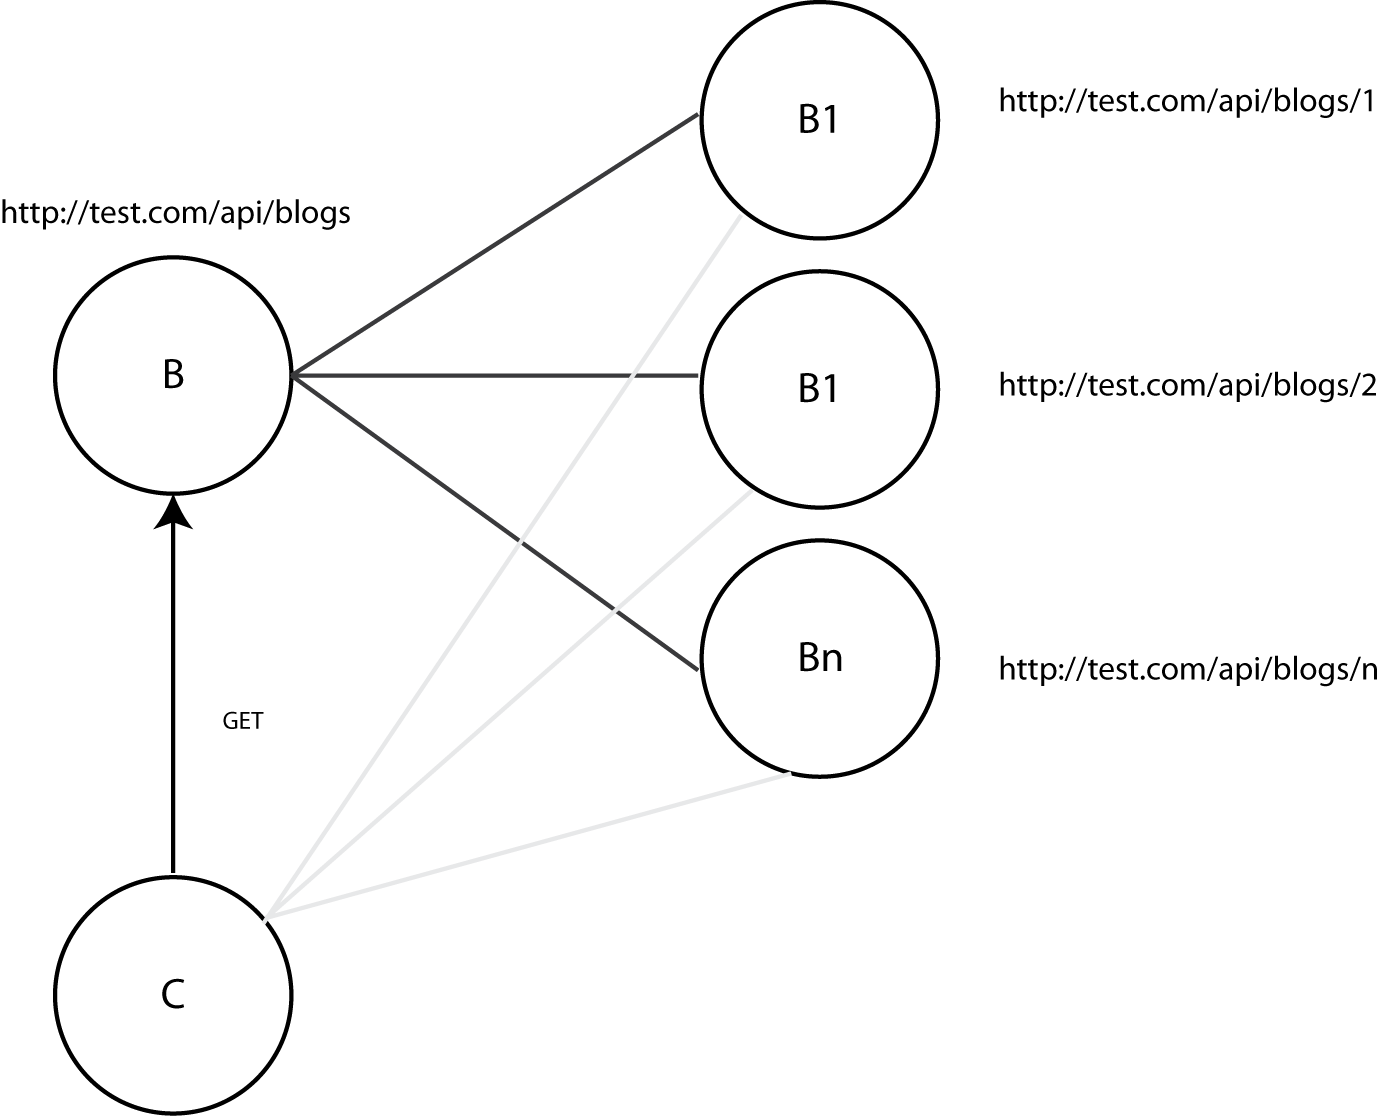
\includegraphics{get_ex.png}
\end{figure}

The symbols used are the following:
\begin{itemize}
  \item Resource $B$ with triple space $TS<B(u)>$ and input channel $l$ with URI \emph{http://test.com/api/blogs}
  \item Client $C$ with triple space $TS<C>$
  \item Type $T$ for the resources of type \emph{http://test.com/api/blog}
  \item Pattern $p$ matching triples of type $T$ in any triple repository
\end{itemize}



\setcounter{equation}{0}
\begin{eqnarray*}
 \ TS<C>,TS<B(u)>\, &\vdash\,&  C\,|\,B(u) \\
 \               &        &          \\
 \ TS<C>,TS<B(u)>\, &\vdash\,& new\,c:[T]\,in\,\overline{l}[GET,p:[T],c:[T]].(rs)c\,|\\
 \               &\,      &(rq)l.[rq = [GET,p_i:[T],c_i[T]]].\overline{c_i}[200,r(u)<p_i>].B(u) \\
 \               &        &          \\
 \ TS<C>,TS<B(u)>\, &\vdash\,& new\,c:[T]\,in\,(rs)c\,|\, \{[GET,p,c]/rq\}.\\
 \               &\,      &[rq = [GET,p_i:[T],c_i:[T]]].\overline{c_i}[200,r(u)<p_i>].B(u) \\
 \               &        &          \\
 \ TS<C>,TS<B(u)>\, &\vdash\,& new\,c:[T]\,in\,(rs)c\,|\, \\
 \               &\,      &[[GET,p,c] = [GET,p_i:[T],c_i:[T]]].\overline{c_i}[200,r(u)<p_i>].B(u) \\
\end{eqnarray*}
\begin{eqnarray*}
\ TS<C>,TS<B(u)>\, &\vdash\,& new\,c:[T]\,in\,(rs)c\,|\,\{p,c/p_i,c_i\} \\
 \               &\,      &\overline{c_i}[200,r(u)<p_i>].B(u) \\
 \               &        &          \\
 \ TS<C>,TS<B(u)>\, &\vdash\,& new\,c:[T]\,in\,(rs)c\,|\,\overline{c}[200,r(u)<p>].B(u) \\
 \               &        &          \\
 \ TS<C>,TS<B(u)>\, &\vdash\,& new\,c:[T]\,in\,(rs)c\,|\,\overline{c}[200,v:[T]].B(u) \\
 \               &        &          \\
 \ TS<C>,TS<B(u)>\, &\vdash\,& \{[200,v]/rs\}\,|\,B(u) \\
 \               &        &          \\
 \ TS<B(u)>\, &\vdash\,& 0\,|\,B(u) \\
\end{eqnarray*}


\subsection{Resource creation}
A client can create new RESTful resources sending the encoded representation of the new resource to a \emph{factory} resource. The new resource will be created by the server and a server chosen URI, under the factory resource URI, will be assigned to it.
In this example, a client send the triple encoded representation of a new resource of type \emph{http://test.com/api/blog} to the factory resource at URI \emph{http://test.com/api/blogs}. The factory resource process creates a new process for the resource, sharing the same triple space, with a new URI under its own URI \emph{http://test.com/api/blogs/3432}, and the channel for the new resource is returned to the client. The triple space for the new process will contain the triple encoded information sent from the client. The triple space of the factory resource will also be updated with the information of the new existent resource.

\begin{figure}[htb!]
\centering%
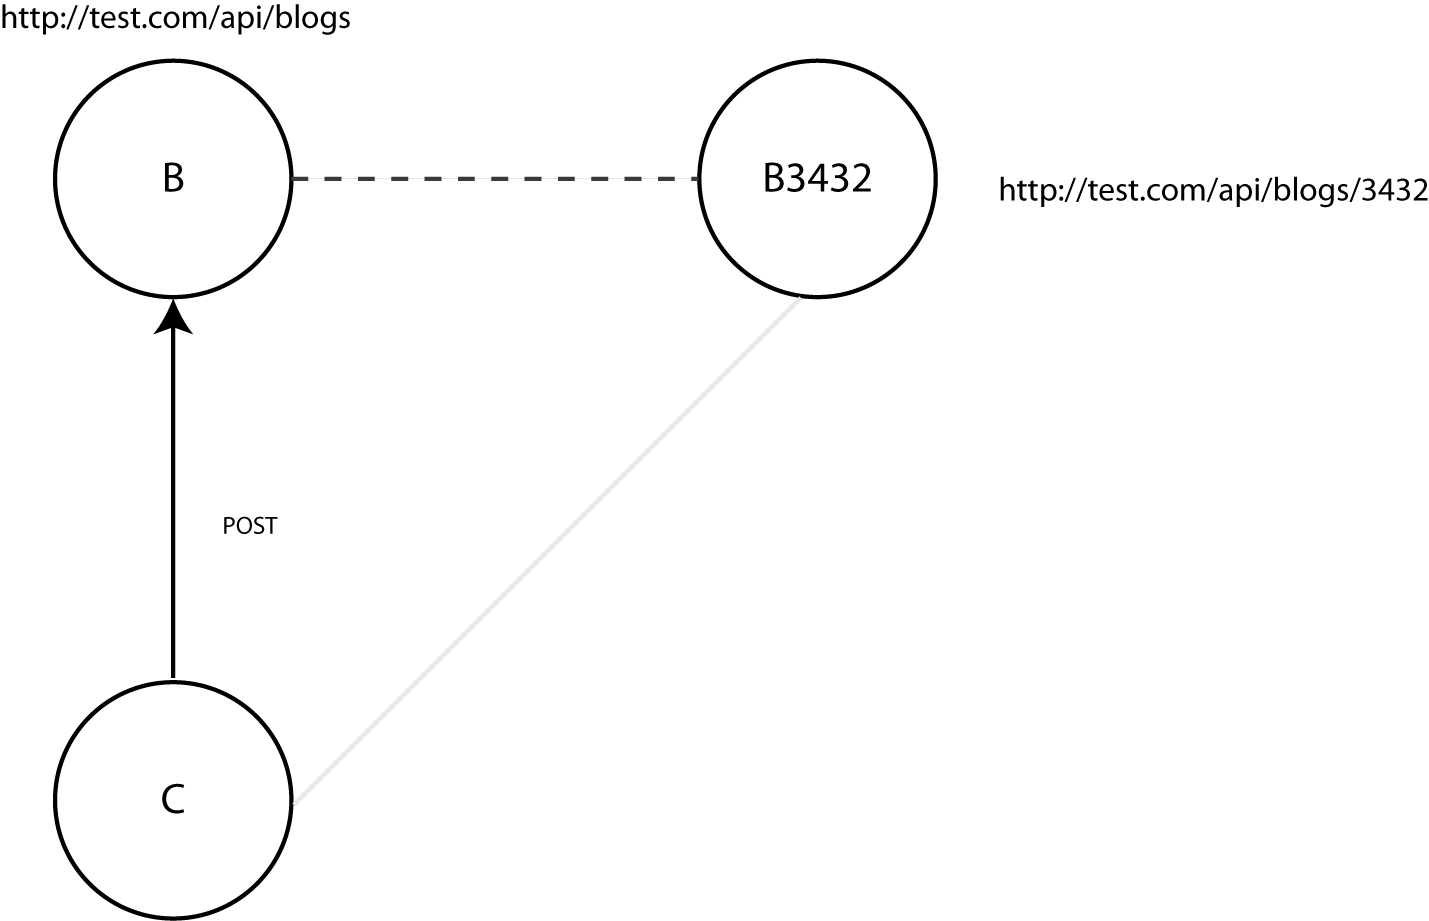
\includegraphics{post_ex.png}
\end{figure}

\setcounter{equation}{0}
\begin{eqnarray*}
 \ TS<C>,TS<B(u)>\, &\vdash\,&  C\,|\,B(u) \\
 \               &        &          \\
 \ TS<C>,TS<B(u)>\, &\vdash\,& new\,c:T\,in\;\overline{l}[POST,p:T,c:T].(rs)c\,|\\
 \               &\,      & new\,r:T\,in\;(rq)l.[rq = [POST,p_i:T,c_i:T]].\\
 \               &        & w(u)<p_i,r>.!B_2(u).\overline{c_i}[201,<p_i,r>].B(u) \\
 \               &        &          \\
 \ TS<C>,TS<B(u)>\, &\vdash\,& new\,c:T\,in\;(rs)c\,|\,new\,r:T\,in\;\\
 \               &\,      & \{[POST,p,c]/rq\}.[rq = [POST,p_i:T,c_i:T]].\\
 \               &        & w(u)<p_i,r>.!B_2(u).\overline{c_i}[201,<p_i,r>].B(u) \\
 \               &        &          \\
 \ TS<C>,TS<B(u)>\, &\vdash\,& new\,c:T\,in\;(rs)c\,|\,new\,r:T\,in\;\\
 \               &\,      & [[POST,p,c] = [POST,p_i:T,c_i:T]].\\
 \               &        & w(u)<p_i,r>.!B_2(u).\overline{c_i}[201,<p_i,r>].B(u) \\
 \               &        &          \\
 \ TS<C>,TS<B(u)>\, &\vdash\,& new\,c:T\,in\;(rs)c\,|\,new\,r:T\,in\;\\
 \               &\,      & \{p,c/p_i,c_i\}.w(u)<p_i,r>.\\
 \               &        & !B_2(u).\overline{c_i}[201,<p_i,r>].B(u) \\
 \               &        &          \\
\end{eqnarray*}
\begin{eqnarray*}
 \ TS<C>,TS<B(u)>\, &\vdash\,& new\,c:T\,in\;(rs)c\,|\,new\,r:T\,in\;\\
 \               &\,      & w(u)<p,r>.!B_2(u).\overline{c}[201,<p,r>].B(u) \\
 \               &        & \\
 \ TS<C>,TS<B(u)>\, &\vdash\,& new\,c:T\,in\;(rs)c\,|\,new\,r:T\,in\;\\
 \               &\,      & w(u)<v:T>.!B_2(u).\overline{c}[201,v:T].B(u) \\
 \               &        & \\
 \ TS<C>,&\vdash\,& new\,c:T\,in\;(rs)c\,|\,new\,r:T\,in\;\\
 \ TS<B(u)>,\cup\{v\}\, &\,      & !B_2(u).\overline{c}[201,v].B(u) \\
 \               &        & \\
 \ TS<C>,TS<B(u)>\, &\vdash\,& new\,c:T\,in\;(rs)c\,|\,new\,r:T\,in\;\\
 \ ,TS<B_2(u)>              &\,      & \overline{c}[201,v].B(u)\,|\,B_2(u) \\
 \               &        & \\
 \ TS<C>,TS<B(u)>,\, &\vdash\,& \{[201,v]/rs\}\,|\,new\,r:T\,in\;\\
 \ TS<B_2(u)>              &\,      & B(u)\,|\,B_2(u) \\
 \               &        & \\
 \ TS<B(u)>,TS<B_2(u)>\, &\vdash\,& 0\,|\,B(u)\,|\,B_2(u) \\
 \               &        & \\
\end{eqnarray*}

\subsection{Resource update}

A client can update any accesible RESTful resource through its URI, sending a new triple encoded representation for the resource in a PUT HTTP request. As a consequence of this request the resource will replace the old triples into its triple space by the new set provided by the client.

\begin{figure}[htb!]
\centering%
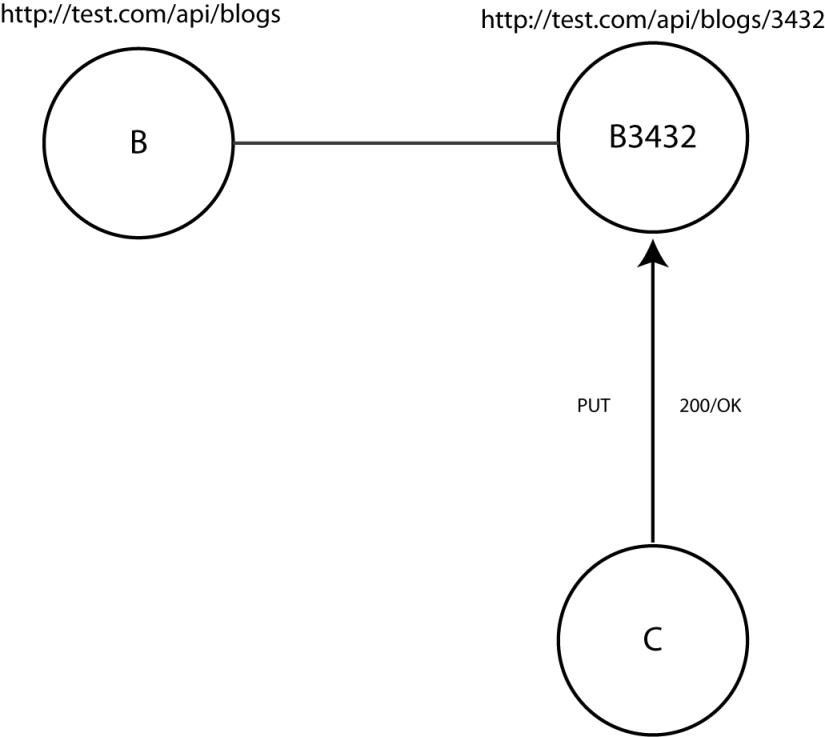
\includegraphics{put_ex.png}
\end{figure}

\setcounter{equation}{0}
\begin{eqnarray*}
 \ TS<C>,TS<B(u)>\, &\vdash\,&  C\,|\,B_2(u)\,|\,B(u) \\
 \ TS<B_2(u)>       &        &          \\
 \               &        &          \\
 \ TS<C>,TS<B(u)>\, &\vdash\,& new\,c:T\,in\;\overline{l}[PUT,v:T,c:T]\,|\\
 \ TS<B_2(u)>       &\,      & (rq)l.[rq = [PUT,v_i:T,c_i:T]].d(u)<r(u)<():T>>.\\
 \               &\,      & .w(u)<v_i>.\overline{c_i}[200,()].B_2(u)\,|\,B(u)\\
 \               &        &          \\
 \ TS<B(u)>,         &\vdash\,& new\,c:T\,in\;0\,|\{[PUT,v,c]/rq\}.\\
 \ TS<B_2(u)>              &\,      & [rq = [PUT,v_i:T,c_i:T]].d(u)<r(u)<():T>>.\\
 \               &\,      & w(u)<v_i>.\overline{c_i}[200,()].B(u)_2\,|\,B(u)\\
 \               &        &          \\
 \ TS<B(u)>,         &\vdash\,& new\,c:T\,in\;0\,|\,[[PUT,v,c]=[PUT,v_i:T,c_i:T].\\
 \ TS<B_2(u)>              &\,      & d(u)<r(u)<():T>>.w(u)<v_i>.\overline{c_i}[200,()].B\\
\end{eqnarray*}
\begin{eqnarray*}
 \               &        &          \\
 \ TS<B(u)>,         &\vdash\,& new\,c:T\,in\;0\,|\,\{v,c/v_i,c_i\}.\\
 \ TS<B_2(u)>              &\,      & d(u)<r(u)<():T>>.w(u)<v_i>.\overline{c_i}[200,()].B_2(u)\,|\\
 \               &        & B(u)\\
 \               &        &          \\
 \ TS<B(u)>,         &\vdash\,& new\,c:T\,in\;0\,|\,\\
 \ TS<B_2(u)>              &      & d(u)<r(u)<():T>>.w(u)<v>.\overline{c}[200,()].B_2(u)\,|\\
 \               &        & B(u)\\
 \               &        &          \\
 \ TS<B(u)>,         &\vdash\,& new\,c:T\,in\;0\,|\,\\
 \ TS<B_2(u)>              &      & d(u)<v_{old}:T>.w(u)<v>.\overline{c}[200,()].B_2(u)\,|\\
 \               &        &  B(u)\\
 \               &        &          \\
 \ TS<B(u)> - \,\{ v_{old} \},        &\vdash\,& new\,c:T\,in\;0\,|\,\\
 \ TS<B_2(u)> - \,\{ v_{old} \}              &      & w(u)<v>.\overline{c}[200,()].B_2(u)\,|\,B(u)\\
 \               &        &          \\
 \ TS<B(u)> \cup \,\{v\},        &\vdash\,& new\,c:T\,in\;0\,|\,\\
 \ TS<B_2(u)> \cup \,\{v\}              &      & \overline{c}[200,()].B_2(u)\,|\,B(u)\\
 \               &        &          \\
 \ TS<B(u)>,TS<B_2(u)>         &\vdash\,& new\,c:T\,in\;0\,|\,\\
 \               &      & \overline{c}[200,()].B_2(u)\,|\,B(u)\\
 \               &       &          \\
 \ TS<B(u)>,TS<B_2(u)>         &\vdash\,& 0\,|\,B_2(u)\,|\,B(u)\\
\end{eqnarray*}


\subsection{Resource destruction}

The destruction of a resource can be achieved by issuing a DELETE HTTP request through the channel identified by the URI of the resource. The resource information will be deleted from the triple space and the process for the resource will terminate.

\begin{figure}[htb!]
\centering%
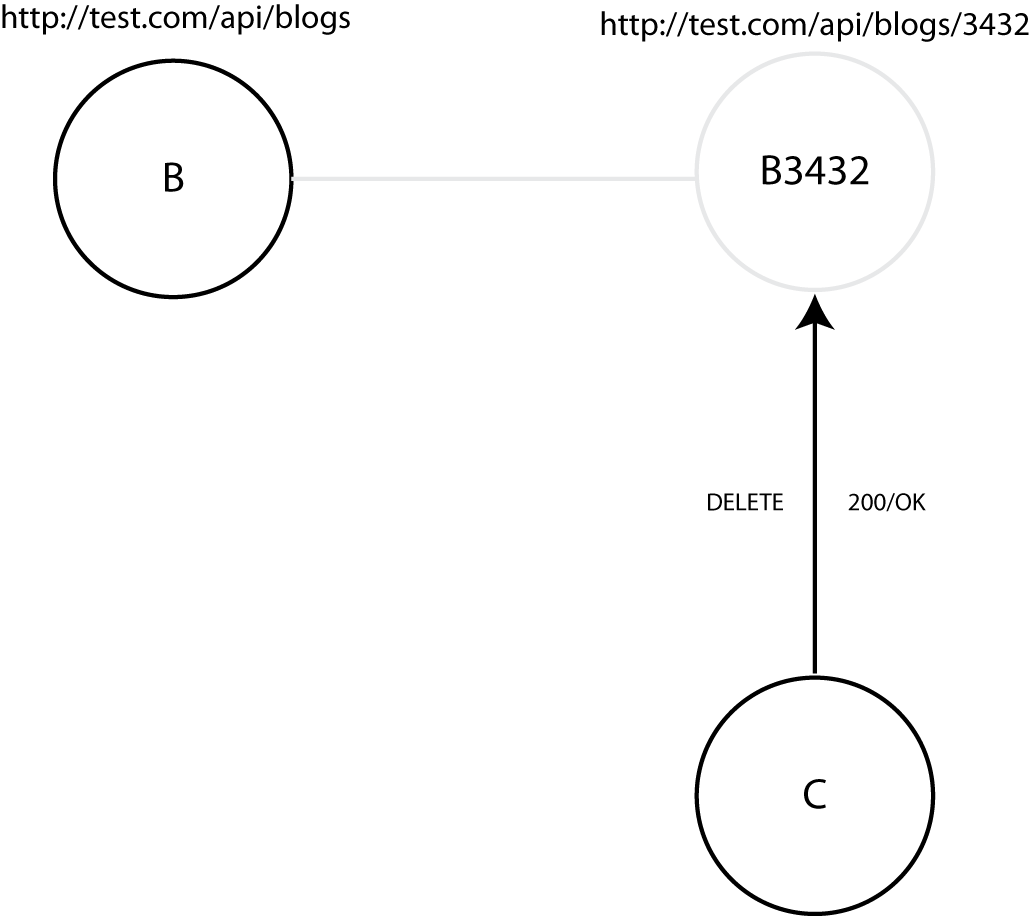
\includegraphics{get_del.png}
\end{figure}

\setcounter{equation}{0}
\begin{eqnarray*}
 \ TS<C>,TS<B_2(u)>\, &\vdash\,&  C\,|\,B_2(u) \\
 \               &        &          \\
 \ TS<C>,TS<B_2(u)>\, &\vdash\,& new\,c:T\,in\;\overline{l}[DELETE,c:T]\,|\\
 \               &\,      & (rq)l.[rq = [DELETE,c_i:T]].d(u)<r(u)<p:T>>.\\
 \               &\,      & \overline{c}[200,()].0\\
 \               &        &          \\
 \ TS<B_2(u)>\, &\vdash\,& new\,c:T\,in\;0\,|\,\{[DELETE,c]/rq\}\\
 \               &\,      & [rq = [DELETE,c_i:T]].d(u)<r(u)<p:T>>.\\
 \               &\,      & \overline{c_i}[200,()].0\\
 \               &        &          \\
 \ TS<B_2(u)>\, &\vdash\,& new\,c:T\,in\;0\,|\,\\
 \               &\,      & [[DELETE,c] = [DELETE,c_i:T]].d(u)<r(u)<p:T>>.\\
 \               &\,      & \overline{c_i}[200,()].0\\
 \               &        &          \\
 \ TS<B_2(u)>\, &\vdash\,& new\,c:T\,in\;0\,|\,\\
 \               &\,      & \{c/c_i\}.d(u)<r(u)<p:T>>.\overline{c_i}[200,()].0\\
 \               &        &          \\
 \ TS<B_2(u)>\, &\vdash\,& new\,c:T\,in\;0\,|\,\\
 \               &\,      & d(u)<r(u)<p:T>>.\overline{c}[200,()].0\\
 \               &        &          \\
\end{eqnarray*}
\begin{eqnarray*}
 \ TS<B_2(u)>\, &\vdash\,& new\,c:T\,in\;0\,|\,\\
 \               &\,      & d(u)<v:T>.\overline{c}[200,()].0\\
 \               &        &          \\
 \ TS<B_2(u)>\,-\,\{v\}\, &\vdash\,& new\,c:T\,in\;0\,|\,\\
 \               &\,      & \overline{c}[200,()].0\\
 \               &        &          \\
 \ &\vdash\,& 0\,|\,0\\
\end{eqnarray*}

\subsection{Clients coordination}

Different client processes sharing the same triple space, can use the blocking operations over the triple space as a mean of coordination in the processing of resources. In this example, there are two process C and D, sharing access to triple space $u_1$, additionally, C has access to triple space $u_2$. C reads a resource P of type T through l, writes it on triple space $u_2$ and on triple space $u_1$. Client D reads the representation of P from $u_1$ and deletes P.
\\
\begin{figure}[htb!]
\centering%
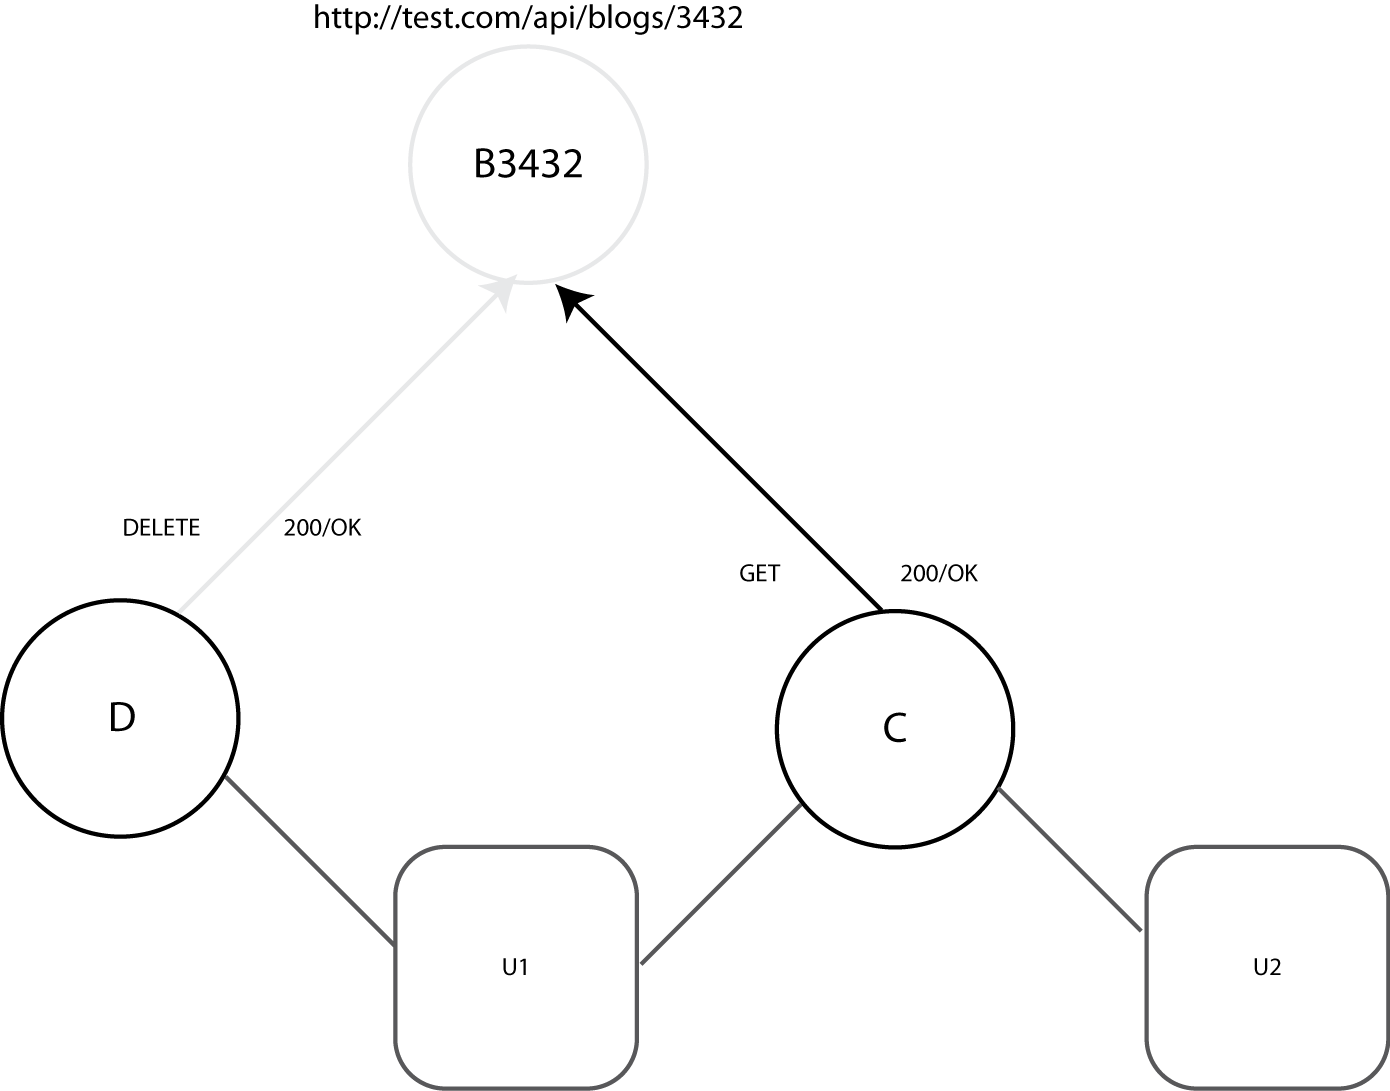
\includegraphics{coord.png}
\end{figure}

\setcounter{equation}{0}
\begin{eqnarray*}
 \ TS<C(u_1,u_2)>,\, &\vdash\,&  P\,|\,C(u_1,u_2)\,|\,D(u_1) \\
 \ TS<D(u_1)>,   &        &          \\
\  TS<P>   &        &          \\
 \               &        &          \\
 \ TS<C(u_1,u_2)>, &\vdash\,& new\,c_1:T,c_2:T,\,in\; (rq)l. \\
 \ TS<D(u_1)>,     &        & [rq = [GET,p_i:T,c_i:T]].\overline{c_i}[200,r<p_i>].P         \\
 \ TS<P>           &        & [rq = [DELETE,(),c_i:T]].d(u)<v_{P}>.\overline{c_i}[200,()].0         \\
 \               &        &    \,|\,      \\
 \               &        &  \overline{l}[GET,p:T,c_1:T].(rs)c_1.[rs = [200,v_o:T]].w(u_2)<v_o>. \\
 \               &        & w(u_1)<v_o>.0        \\
 \               &        &    \,|\,      \\
 \               &        &  br(u_1)<p:T>.\overline{l}[DELETE,(),c_2].0 \\
 \               &        &          \\
 \ TS<C(u_1,u_2)>, &\vdash\,& new\,c_1:T,c_2:T,\,in\; \{[GET,p,c_1]/rq\}. \\
 \ TS<D(u_1)>,     &        & [[GET,p,c_1] = [GET,p_i:T,c_i:T]].\overline{c_i}[200,r<p_i>].P         \\
 \ TS<P>              &        &    \,|\,      \\
 \               &        &  (rs)c_1.[rs = [200,v_o:T]].w(u_2)<v_o>. \\
 \               &        & w(u_1)<v_o>.0        \\
 \               &        &    \,|\,      \\
 \               &        &  br(u_1)<p:T>.\overline{l}[DELETE,(),c_2].0 \\
 \               &        &          \\
 \ TS<C(u_1,u_2)>, &\vdash\,& new\,c_1:T,c_2:T,\,in\; \\
 \ TS<D(u_1)>,     &        & \{ p,c_1 / p_i, c_i \}.\overline{c_i}[200,r<p_i>].P         \\
 \ TS<P>           &        &    \,|\,      \\
 \               &        &  (rs)c_1.[rs = [200,v_o:T]].w(u_2)<v_o>. \\
 \               &        & w(u_1)<v_o>.0        \\
 \               &        &    \,|\,      \\
 \               &        &  br(u_1)<p:T>.\overline{l}[DELETE,(),c_2].0 \\
 \               &        &          \\
\end{eqnarray*}
\begin{eqnarray*}
 \ TS<C(u_1,u_2)>, &\vdash\,& new\,c_1:T,c_2:T,\,in\; \\
 \ TS<D(u_1)>,     &        & \overline{c_1}[200,r<p>].P         \\
 \ TS<P>            &        &    \,|\,      \\
 \               &        &  (rs)c_1.[rs = [200,v_o:T]].w(u_2)<v_o>. \\
 \               &        & w(u_1)<v_o>.0        \\
 \               &        &    \,|\,      \\
 \               &        &  br(u_1)<p:T>.\overline{l}[DELETE,(),c_2].0 \\
 \               &        &          \\
 \ TS<C(u_1,u_2)>, &\vdash\,& new\,c_1:T,c_2:T,\,in\;  \\
 \ TS<D(u_1)>,     &        & \overline{c_1}[200,v:T].P         \\
 \ TS<P>            &        &    \,|\,      \\
 \               &        &  (rs)c_1.[rs = [200,v_o:T]].w(u_2)<v_o>. \\
 \               &        & w(u_1)<v_o>.0        \\
 \               &        &    \,|\,      \\
 \               &        &  br(u_1)<p:T>.\overline{l}[DELETE,(),c_2].0 \\
 \               &        &          \\
 \ TS<C(u_1,u_2)>, &\vdash\,& new\,c_1:T,c_2:T,\,in\; \\
 \ TS<D(u_1)>,   &        & P        \\
 \ TS<P>         &        &    \,|\,      \\
 \               &        & \{[200,v] / rs\}.[rs = [200,v_o:T]].w(u_2)<v_o>. \\
 \               &        & w(u_1)<v_o>.0        \\
 \               &        &    \,|\,      \\
 \               &        &  br(u_1)<p:T>.\overline{l}[DELETE,(),c_2].0 \\
 \               &        &          \\
 \ TS<C(u_1,u_2)>, &\vdash\,& new\,c_1:T,c_2:T,\,in\; (rq)l.[rq = [DELETE,(),c_i:T]].\\
 \ TS<D(u_1)>,   &        & d(u)<v_{P}>.\overline{c_i}[200,()].0         \\
 \ TS<P>              &        & [[200,v] = [200,v_o:T]].w(u_2)<v_o>. \\
 \               &        & w(u_1)<v_o>.0        \\
 \               &        &    \,|\,      \\
 \               &        &  br(u_1)<p:T>.\overline{l}[DELETE,(),c_2].0 \\
 \               &        &          \\
\end{eqnarray*}
\begin{eqnarray*}
 \ TS<C(u_1,u_2)>, &\vdash\,& new\,c_1:T,c_2:T,\,in\; (rq)l.[rq = [DELETE,(),c_i:T]].\\
 \ TS<D(u_1)>,   &        & d(u)<r(u)<p_i:T>>.\overline{c_i}[200,()].0         \\
 \ TS<P>         &        &    \,|\,      \\
 \               &        & \{v / v_o \}.w(u_2)<v_o>.w(u_1)<v_o>.0 \\
 \               &        &    \,|\,      \\
 \               &        &  br(u_1)<p:T>.\overline{l}[DELETE,br(u_1)<p:T>,c_2].0 \\
 \               &        &          \\
 \ TS<C(u_1,u_2)>, &\vdash\,& new\,c_1:T,c_2:T,\,in\; (rq)l.[rq = [DELETE,(),c_i:T]].\\
 \ TS<D(u_1)>,   &        & d(u)<r(u)<p_i:T>>.\overline{c_i}[200,()].0         \\
 \ TS<P>         &        &    \,|\,      \\
 \               &        & w(u_2)<v>.w(u_1)<v>.0 \\
 \               &        &    \,|\,      \\
 \               &        &  br(u_1)<p:T>.\overline{l}[DELETE,(),c_2].0 \\
 \               &        &          \\
 \ TS<C(u_1,u_2)>\,\cup\,\{v\}, &\vdash\,& new\,c_1:T,c_2:T,\,in\; (rq)l.[rq = [DELETE,(),c_i:T]]. \\
 \ TS<D(u_1)>,   &        & d(u)<r(u)<p_i:T>>.\overline{c_i}[200,()].0         \\
 \ TS<P>         &        &    \,|\,      \\
 \               &        & w(u_1)<v>.0 \\
 \               &        &    \,|\,      \\
 \               &        &  br(u_1)<p:T>.\overline{l}[DELETE,(),c_2].0 \\
 \               &        &          \\
 \ TS<C(u_1,u_2)>\,\cup\,\{v\}, &\vdash\,& new\,c_1:T,c_2:T,\,in\; (rq)l.[rq = [DELETE,(),c_i:T]]. \\
 \ TS<D(u_1)>,   &        & d(u)<r(u)<p_i:T>>.\overline{c_i}[200,()].0         \\
 \ TS<P>         &        &    \,|\,      \\
 \               &        & 0 \\
 \               &        &    \,|\,      \\
 \               &        &  br(u_1)<p:T>.\overline{l}[DELETE,(),c_2].0 \\
 \               &        &          \\
 \ TS<D(u_1)>, &\vdash\,& new\,c_1:T,c_2:T,\,in\; (rq)l.[rq = [DELETE,(),c_i:T]].\\
 \ TS<P>   &        & d(u)<r(u)<p_i:T>>.\overline{c_i}[200,()].0         \\
 \         &        &    \,|\,      \\
 \               &        & 0 \\
 \               &        &    \,|\,      \\
 \               &        &  br(u_1)<p:T>.\overline{l}[DELETE,(),c_2].0 \\
 \               &        &          \\
\end{eqnarray*}
\begin{eqnarray*}
 \ TS<D(u_!)>, &\vdash\,& new\,c_1:T,c_2:T,\,in\; (rq)l.[rq = [DELETE,(),c_i:T]]. \\
 \ TS<P>   &        & d(u)<r(u)<p_i:T>>.\overline{c_i}[200,()].0         \\
 \         &        &    \,|\,      \\
 \               &        & 0 \\
 \               &        &    \,|\,      \\
 \               &        & br(u_1)<v>.\overline{l}[DELETE,(),c_2].0 \\
 \               &        &          \\
 \ TS<D(u_1)>, &\vdash\,& new\,c_1:T,c_2:T,\,in\; (rq)l.[rq = [DELETE,(),c_i:T]]. \\
 \ TS<P>   &        & d(u)<r(u)<p_i:T>>.\overline{c_i}[200,()].0         \\
 \         &        &    \,|\,      \\
 \               &        & 0 \\
 \               &        &    \,|\,      \\
 \               &        & \overline{l}[DELETE,(),c_2].0 \\
 \               &        &          \\
 \ TS<P> &\vdash\,& new\,c_1:T,c_2:T,\,in\; \{[DELETE,(),c_2] / rq \}. \\
 \    &        & [rq = [DELETE,(),c_i:T]].d(u)<r(u)<p_i:T>>.\overline{c_i}[200,()].0         \\
 \         &        &    \,|\,      \\
 \               &        & 0 \\
 \               &        &    \,|\,      \\
 \               &        & 0 \\
 \               &        &          \\
 \ TS<P> &\vdash\,& new\,c_1:T,c_2:T,\,in\; [[DELETE,(),c_2] = [DELETE,(),c_i:T]].\\
 \    &        & d(u)<r(u)<p_i:T>>.\overline{c_i}[200,()].0         \\
 \         &        &    \,|\,      \\
 \               &        & 0 \\
 \               &        &    \,|\,      \\
 \               &        & 0 \\
 \               &        &          \\
 \ TS<P> &\vdash\,& new\,c_1:T,c_2:T,\,in\; \\
 \    &        & \{c_2 / c_i\}.d(u)<r(u)<p_i:T>>.\overline{c_i}[200,()].0         \\
 \          &        &    \,|\,      \\
 \               &        & 0 \\
 \               &        &    \,|\,      \\
 \               &        & 0 \\
\end{eqnarray*}
\begin{eqnarray*}
 \               &        &          \\
 \ TS<P> &\vdash\,& new\,c_1:T,c_2:T,\,in\; \\
 \   &        & d(u)<v>.\overline{c_2}[200,()].0         \\
 \          &        &    \,|\,      \\
 \               &        & 0 \\
 \               &        &    \,|\,      \\
 \               &        & 0 \\
 \               &        &          \\
 \ TS<P>\,-\,\{v\} &\vdash\,& new\,c_1:T,c_2:T,\,in\; \\
 \    &        & \overline{c_2}[200,()].0         \\
 \         &        &    \,|\,      \\
 \               &        & 0 \\
 \               &        &    \,|\,      \\
 \               &        & 0 \\
 \               &        &          \\
 \  &\vdash\,& new\,c_1:T,c_2:T,\,in\; \\
 \    &        & 0         \\
 \         &        &    \,|\,      \\
 \               &        & 0 \\
 \               &        &    \,|\,      \\
 \               &        & 0 \\
 \               &        &          \\
\end{eqnarray*}

\section{Extensions}
Some possible extensions to easily model some aspects of the services consumption process are discussed in this section.

\subsection{Headers and authentication}
In RESTful architectures, HTTP protocol headers are used along with the request and response bodies to exchange useful information between clients and servers. In the proposed version of the calculus, the only use of headers has been the returning of a response code from the server process.\\
It may be interesting to include support for including collection of headers in the messages exchanged between processes. We could define the messages as:\\
\begin{equation*}
m\,::=\,[VERB,[(k,v)]:[H],v:T,c:T]
\end{equation*}
\\Where $[(k,v)]$ is a collection of headers with keys $k$ and value $v$. The information sent in the headers of the request can be used to define primitives for authentication or conditional request.

\subsection{Metaresources}
In the proposed calculus types have been used to add aditional information to the channels, patterns and messages exchanged. Information about these types are provided beforehand something that is not a realistic assumption for actual implementations of the calculus, where clients will need some kind of mechanism to retrieve the type associated to the URIs and triples returned from these URIs. A possible solution to this problem is the definition of special resources capable of describing other resources, offering information about the types of the resources described, channels and operations available on them.\\
The formalization of these metaresources can be achieved extending the calculus with some extra syntax:
\begin{itemize}
  \item $r:R<T>$: a set of triples describing a resource of type $T$.
  \item $<r:R<T>,v:T>$: applying a description of type $T$ to a resource of type $T$.
\end{itemize}
The result of applying the description to a resource is a set of datatype properties and object properties, where the object properties, consisting on typed URIs, can be used by the client to retrieve related resources.

\section{Conclusions}
In this document a formal system for describing RESTful web servies and the interaction between clientes and servers has been described. The calculus describes what we call semantic RESTful web services since all the representation of resources and communication channels are typed offering metainformation about the resources offered. The calculus is also based on ideas extracted from triple space computing offering a common representation for the values exchanged and communication operations between processes based on triple spaces. Each resource representation is retrieved or sent as sets of triples or patters for triples retrieval and each process has one or more associated triple spaces where these triples are stored and modified.\\
The calculus proposed can be useful when addressing important theoretical questions about distributed systems based on RESTful web services such as whether two systems are equivalent.\\
The calculus can also serve as the solid foundation for a software implementation of a system capable of automating the building and composition of RESTful web services.


